\section[Aplicación]{Aplicación web}


Como se establecio en el obejetivo de este trabajo (ver \Tref{cp1:objetivoG}{Objetivo general}), se ha desarrollado una aplicación para recolectar y clasificar noticias, las cuales son mostrados en un entorno web. En esta sección se explica el proceso de funcionamiento de la aplicación web.\\



La aplicación esta dieseñada en 4 etapas, las cuales son mostradas en la Figura \ref{fig:procesoAppWeb}, donde la etapa \textbf{Selección} describe las secciones disponibles para obtener noticias; la etapa \textbf{Recolectar} muestra la integración de los \textit{crawlwers} en la herramienta; la etapa \textbf{Clasificar} hace uzo del modelo clasificador desarrollado en la sección anterior y para concluir, la etapa \textbf{Mostrar resultados} describe la forma en que los datos son presentados al usuario. A continuación se explica a detalla cada una las tareas.




\begin{figure}[H]
	\centering
	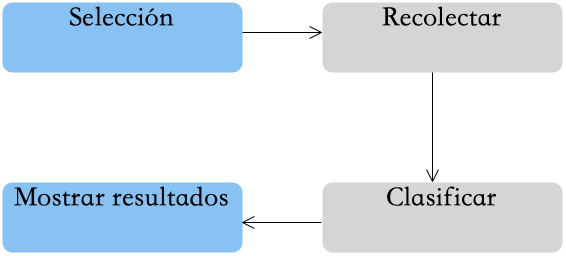
\includegraphics[scale=0.55]{imagenes/Capitulo5/AplicacionWeb/ProcesoAplicacionWeb.png}
	\caption{Etapas de la aplicación web}
	\label{fig:procesoAppWeb}
\end{figure}

%
% este proceso se llevará a cabo la primera vez que se seleccione una sección o en el caso de que %hayan transucurrido 4 horas de la última vez que se utilizó el sistema.%
%\\%
%
%\begin{figure}[H]
%	\centering
%	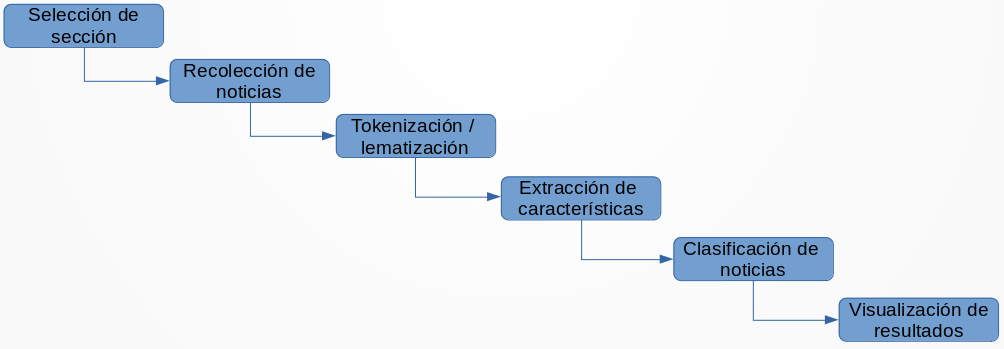
\includegraphics[scale=0.3]{imagenes/Capitulo5/procesoRecoleccionClasificacion.png}
%	\caption{Etapas de la aplicación web}
%	\label{fig:procesoAppWeb}
%\end{figure}
%

\subsection{Selección}


Esta etapa permite elegir al usuario el tipo de noticias a buscar. La aplicación comienza en una pantalla inicial, donde se muestra un menú con las opciones \textbf{Inicio}, \textbf{Cultura}, \textbf{Deportes}, \textbf{Economía}, \textbf{Política}, \textbf{Ciencia y Tecnología}, estas categorías (excluyendo \textbf{Inicio}) son las secciones permitidas para recolectar noticias, como se muestra la el Figura \ref{fig:PantallaInicio}. Cabe mencionar que la opción \textbf{Inicio}, permite regresar a la pantalla principal.\\


\begin{figure}[H]
\centering

\includegraphics[scale=0.29]{imagenes/Capitulo5/pantallaPrincipal.png}
\caption{Pantalla de Inicio.}
\label{fig:PantallaInicio}
\end{figure}

Después de elegir una sección, se muestra el mensaje \textbf{En proceso de recolección y clasificación}, como se visualiza en la Figura \ref{fig:loading}, el cual informa que las etapas \textbf{Recolectar} y \textbf{Clasificar} están en proceso, además cuando se muestra este mensaje no se puede seleccionar otra secciones hasta que el proceso concluya. Cabe destacar que el proceso continua de forma normal si se cumplen las siguientes condiciones:

\begin{enumerate}
	\item \textbf{Primera vez}: Esta condición hace referencia a la etapa \textbf{selección}, es decir cuando es la primera vez que se ha selecciona una sección, se debe proceder con las siguientes etapas

	\item \textbf{Límite de periodo}: Esta condición define 4 horas como el periodo de recolección, es decir cuando se ha solicitado mostrar las noticias de una sección y ha transcurrido 4 horas des de la última petición, se debe proceder con las siguientes etapas
\end{enumerate}	

Como consecuencia de no cumplirse estas condiciones, las etapas \textbf{Recolectar y Clasificar} no son iniciadas, debido a que los artículos con su clasificación correspondiente se encuentran almacenados en el sistema, por esta razón se procede directamente con la etapa \textbf{Mostrar resultado}.\\

\begin{figure}[H]
\centering
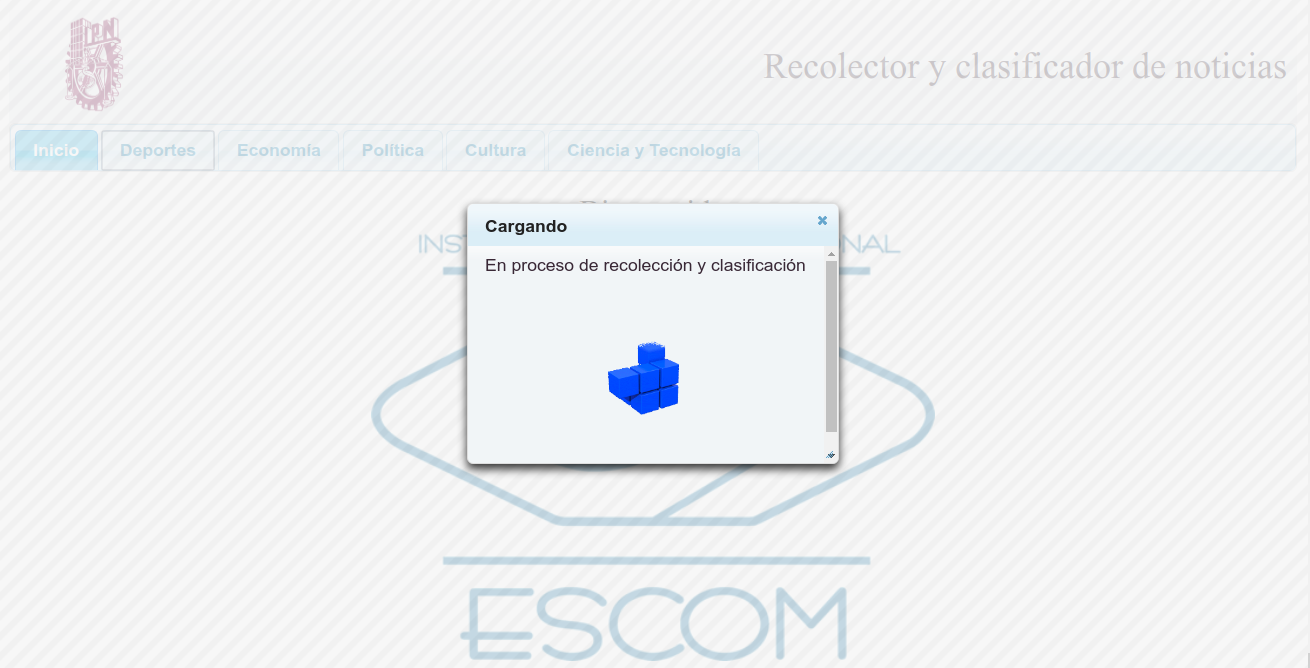
\includegraphics[scale=0.29]{imagenes/Capitulo5/mensajeEspera.png}
\caption{Mensaje de espera.}
\label{fig:loading}
\end{figure}


\subsection{Recolectar}


Esta etapa genera un subproceso el cual activa un script (desarrollado en \textbf{Python 3}) el cual activa la recolección de noticias en los sitio web definidos previamente (ver \Tref{cp5:sitiosWeb}{Sitios web}), la información que se obtiene de cada artículo es la siguiente:

\begin{itemize}
	\item \textbf{URL de la noticia}
	\item \textbf{Título}
	\item \textbf{Fecha}
	\item \textbf{Autor}
	\item \textbf{Descripción} (Existen sitios web, donde las noticias no cuentan con una descripción)
	\item \textbf{Noticia}
\end{itemize}

La extracción de las noticias se hace en la página principal de los sitios web. Cabe destacar que en el proceso de recolección se valida que las noticias contengan al menos 180 palabras, de lo contrario no se extrae. Ademas se ha definido un tiempo máximo de espera en esta etapa, el cual es de 84 segundos, después de concluir el periodo y haber recolectado la información, se procede con la etapa de \textbf{Clasificación}, de lo contrario si no se recolecto ninguna noticia se muestra el mensaje \textbf{Se ha agotado el tiempo de espera, no se han encontrado noticias, intentar mas tarde} (como se visualiza en la Figura \ref{fig:notNoRec}) y se detiene el proceso.

\begin{figure}[H]
\centering
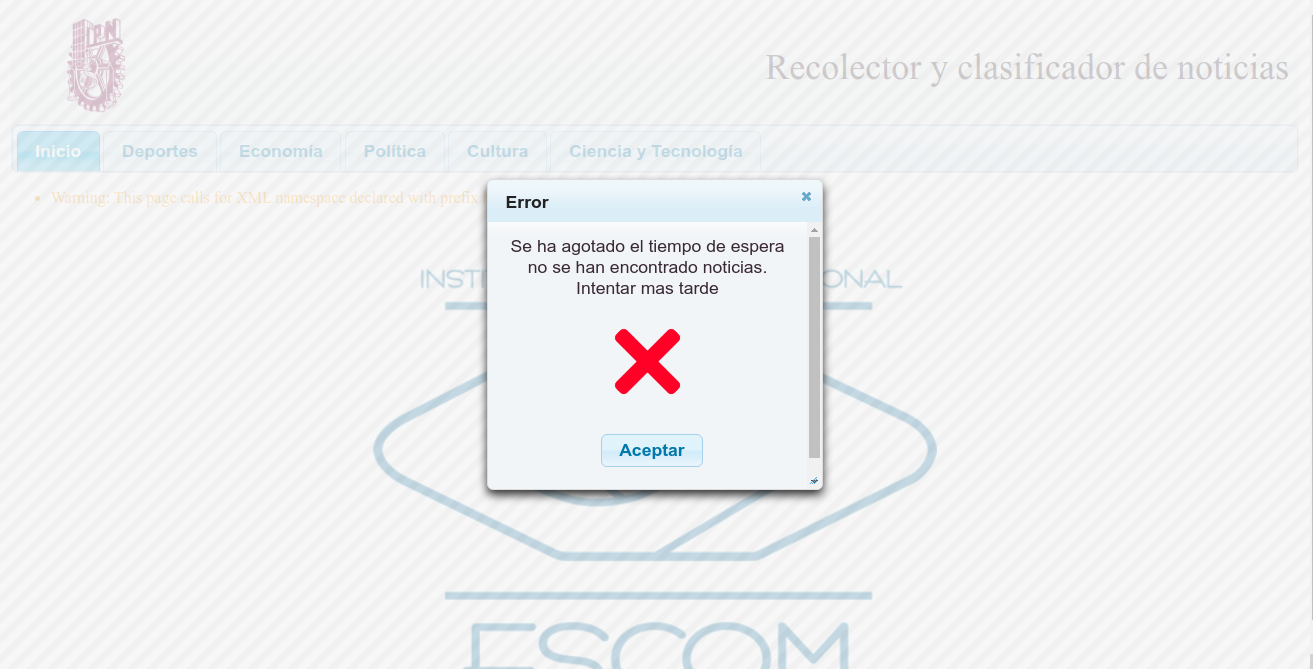
\includegraphics[scale=0.29]{imagenes/Capitulo5/errorConectividad.png}
\caption{Mensaje de error en la recolección}
\label{fig:notNoRec}
\end{figure}

\subsection{Clasificar}

Después de recolectar las noticias se inicia la etapa de clasificación, el cual esta conformado por 5 tareas (como se muestra en la Figura \ref{clasificacion}). Esta etapa genera un subproceso para ejecutar un script desarrollado en \textbf{Python 3}, el cual esta encargado de llevar acabo cada tarea. Cabe destacar que el proceso de clasificación solo utiliza el contenido de la noticia, los demás datos no son necesarios en esta etapa. A continuación se explica cada subtareas.

\begin{figure}[H]
\centering
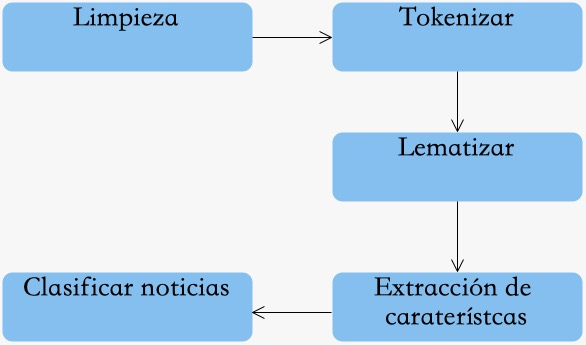
\includegraphics[scale=0.55]{imagenes/Capitulo5/AplicacionWeb/PreprocesamientoWeb.png}
\caption{Proceso de clasificación}
\label{fig:cp5:clasificacion}
\end{figure}

\begin{enumerate}

	\item \textbf{Limpieza}: En esta etapa se eliminan todos los saltos de línea
	\item \textbf{Tokenizar}: Consiste en separar el texto en sus elementos mínimos por un espacio (ver \Tref{cp5:tokenizacion}{Tokenizar})
	\item \textbf{Lematrizer}: Proceso que reduce cada una de las palabras tokenizadas en lemas(ver \Tref{cp5:lematizacion}{Lematizar})
	\item \textbf{Extracción de características}: Se extrae palabras (características) con base al vocabulario definido al final de la etapa de entrenamiento (ver \ref{}), para crear un espacio vectorial por cada noticia (esta es la representación que el algoritmo entiende). Cabe destacar que las características son extraídas de forma binaria (ver \Tref{cp5:extraccion}{Extracción de características})
	\item \textbf{Clasificar}: Al final de la sección \textbf{Entrenamiento} se persistió el modelo clasificador (ver \Tref{cp5:persistencia}{Persistencia}) el cual esta basado en el algoritmo \textbf{Maquinas de soporte vectorial} (ver \Tref{cp3:msv}{MSV}). Esta tarea utiliza el clasificador el cual recibe como entrada los vectores de características(los cuales representan el contenido de cada artículo) y como salida brinda la clasificación del conjunto de noticias, y son almacenadas por sección en un archivo \textbf{CSV}

\end{enumerate}


\subsection{Mostrar resultados}


Cuando el proceso de clasificación ha concluido se muestra el mensaje \textbf{Noticias listas para ser mostradas}, donde el usuario tiene la opción de elegir si desea visualizar las noticias o cancelar, como se visualiza en la Figura \ref{fig:notClass}.

\begin{figure}[H]
\centering
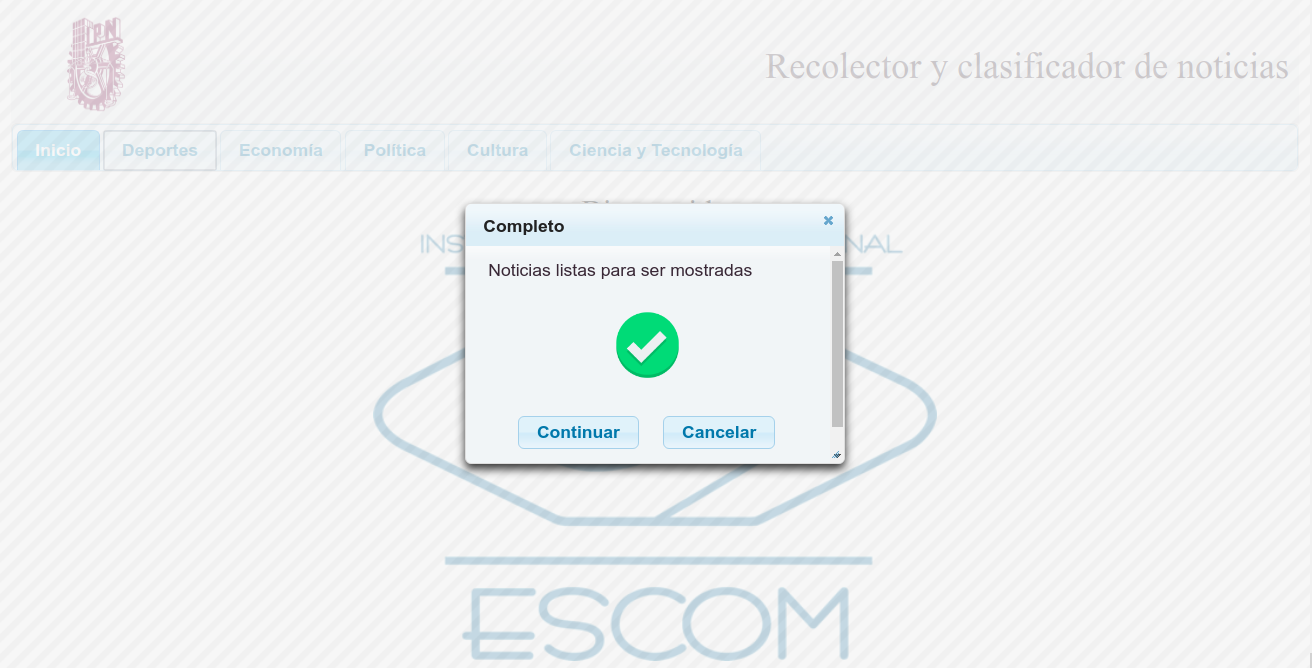
\includegraphics[scale=0.29]{imagenes/Capitulo5/noticiasListasParaSerMostradas.png}
\caption{Mensaje que se muestra una vez clasificadas las noticias}
\label{fig:notClass}
\end{figure}

Si el usuario ha presionado la opción \textbf{continuar}, los artículos clasificados de la sección elegida son obtenidos. En la pantalla principal, las noticias se muestran por fecha de publicación, la información que se muestra es: \textbf{título de la noticia}, \textbf{resumen de la noticia}(de contar con ello), \textbf{autor} y finalmente la \textbf{fecha de publicación}. Como se muestra en la Figura \ref{fig:vistaNoticias}.

\begin{figure}[H]
\centering
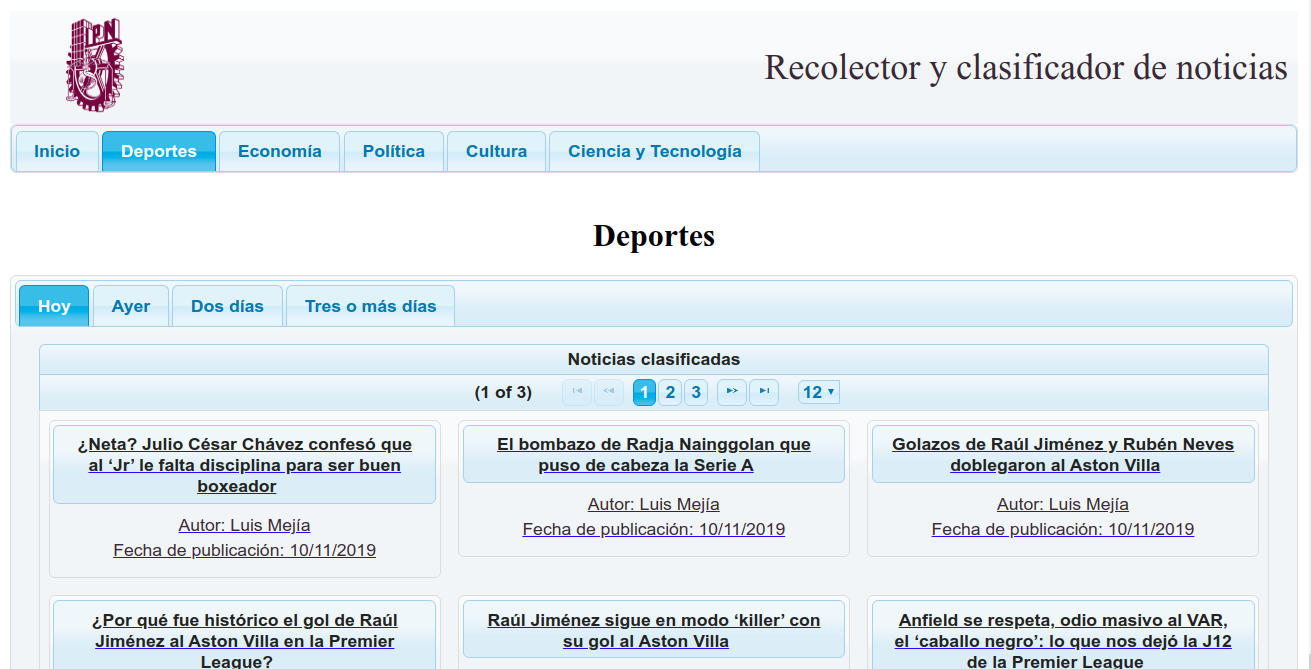
\includegraphics[scale=0.29]{imagenes/Capitulo5/noticiasDeHoy.png}
\caption{Vista de las noticias recolectadas.}
\label{fig:vistaNoticias}
\end{figure}


Si el usuario desea visualizar noticias del dia de ayer, la vista que tendrá se muestra en la Figura \ref{fig:vistaNoticiasAyer}.
\\
\begin{figure}[H]
\centering
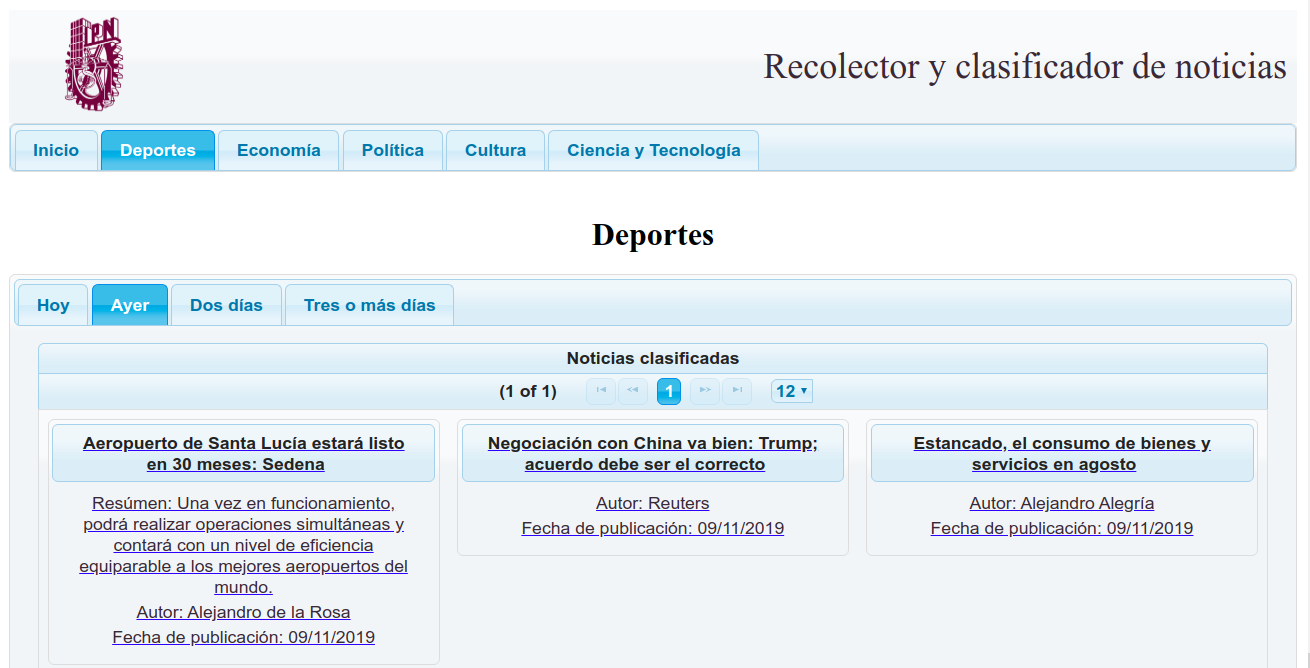
\includegraphics[scale=0.29]{imagenes/Capitulo5/noticiasDeAyer.png}
\caption{Vista de las noticias recolectadas del día de ayer.}
\label{fig:vistaNoticiasAyer}
\end{figure}

Existe la posibilidad de que no se recolecten noticias, si después de 84 segundos, no se realizó la recolección de noticias debido a una falla con nuestra conectividad de Internet, la pantalla que el usuarió tendrá se muestra en la Figura 
